\addtocontents{toc}{\protect\setcounter{tocdepth}{1}}
\chapter{Recurrent Neural Networks (RNN) \& Sequence Models}

\section{Introduction to Sequence Data \& Word Representations}

Standard Feedforward Neural Networks (ANNs) and Convolutional Neural Networks (CNNs) assume that all input samples are independent and identically distributed (i.i.d.). However, real-world data such as text, speech, time-series measurements, financial stocks, and genomic sequences possess temporal or sequential structure where order matters fundamentally.

Before feeding discrete categorical entities like text words into neural networks, they must be converted into numerical vectors.

\subsection{Encoding Strategies: One-Hot vs. Integer Encoding}

Consider two basic approaches to numerical encoding:

\begin{enumerate}
    \item \textbf{Integer Encoding:} Assigning an arbitrary integer ID to each unique word in a dictionary (e.g., $\text{US} = 1, \text{China} = 2, \text{India} = 3$).
    
    \begin{propertybox}[Failure of Integer Encoding]
    Integer encoding introduces arbitrary algebraic ordering and distance relationships that do not exist in language:
    \begin{equation}
    \text{US} + \text{China} = 1 + 2 = 3 = \text{India}
    \end{equation}
    Neural network layers multiply inputs by continuous weights ($W \cdot x$), turning these arbitrary numerical relationships into invalid semantic biases.
    \end{propertybox}

    \item \textbf{One-Hot Encoding:} Representing each word as a sparse binary vector in $\mathbb{R}^V$ (where $V$ is vocabulary size) with a single $1$ at the word's index and $0$ elsewhere:
    \begin{equation}
    e_{\text{king}} = \begin{bmatrix} 1 \\ 0 \\ 0 \\ \vdots \\ 0 \end{bmatrix}, \quad
    e_{\text{queen}} = \begin{bmatrix} 0 \\ 1 \\ 0 \\ \vdots \\ 0 \end{bmatrix}, \quad
    e_{\text{apple}} = \begin{bmatrix} 0 \\ 0 \\ 1 \\ \vdots \\ 0 \end{bmatrix}
    \end{equation}
\end{enumerate}

\begin{advbox}[One-Hot Encoding Limitations]
\textbf{Limitations of One-Hot Vectors:}
\begin{itemize}
    \item \textbf{High Dimensionality \& Sparsity:} For a modest vocabulary size $V = 100,000$, every word vector has length $100,000$ with $99.999\%$ zeros (e.g., $x \in \mathbb{R}^{100000}$).
    \item \textbf{Lack of Semantic Similarity:} Standard basis vectors are orthogonal:
    \begin{equation}
    e_i^T e_j = 0 \quad \forall i \neq j \implies \text{Cosine Similarity}(\text{king}, \text{queen}) = 0
    \end{equation}
    The network cannot infer that "king" and "queen" share semantic properties while "apple" is distinct.
\end{itemize}
\end{advbox}

\subsection{Text Data Processing Pipeline}

To prepare raw text for recurrent neural networks, data passes through a 7-step processing pipeline:

\begin{enumerate}
    \item \textbf{Tokenization:} Split raw text into tokens (words or characters), e.g., \textit{"to be or not to be"}.
    \item \textbf{Count Word Frequencies:} Compute occurrence statistics across the text corpus.
    \item \textbf{Sort by Frequency:} Order tokens from highest frequency to lowest.
    \item \textbf{Build Vocabulary:} Select the top $V$ most frequent words to construct the dictionary.
    \item \textbf{Assign Word Indices:} Map each unique token to an integer ID ($1 \dots V$).
    \item \textbf{Vector Encoding:} Convert integer IDs to One-Hot vectors or dense Embeddings.
    \item \textbf{Unknown Word Token:} Map out-of-vocabulary words to a special unknown token, $\langle \text{UNK} \rangle$.
\end{enumerate}
\begin{figure}[H]
    \centering
    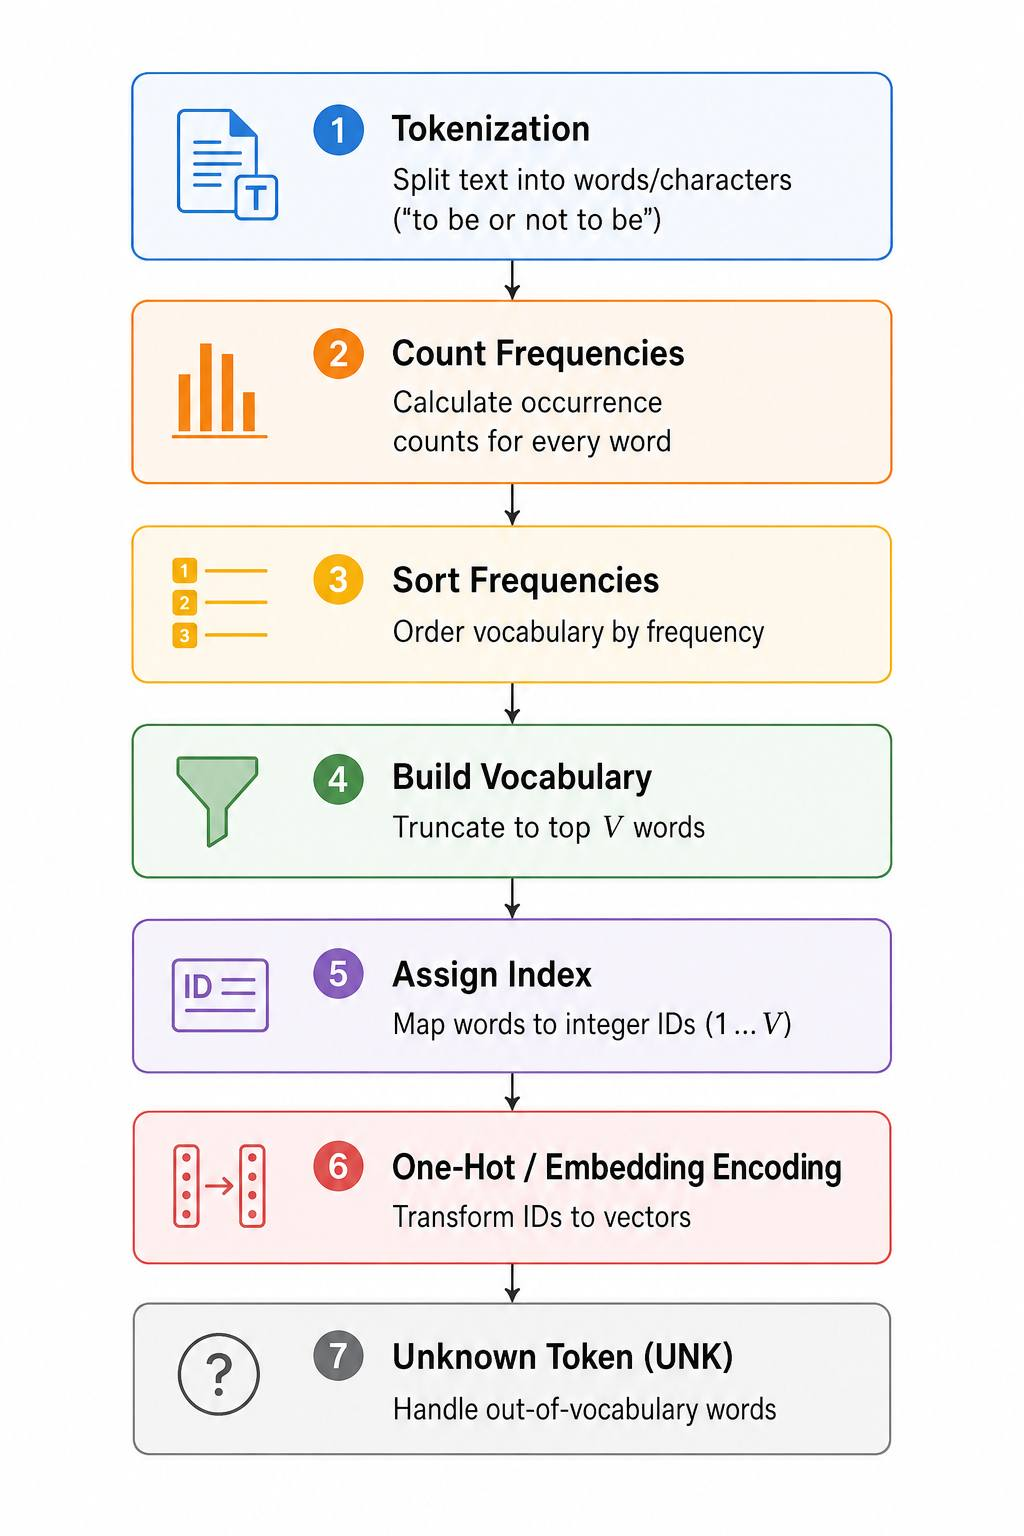
\includegraphics[width=0.95\textwidth]{figures/last.jpg}
\end{figure}

\subsection{Word Embedding Vectors}

Word Embeddings resolve the limitations of One-Hot encoding by projecting discrete words into a dense, low-dimensional continuous vector space $\mathbb{R}^d$ (typically $d \ll V$, e.g., $d \in [50, 300]$).

\begin{equation}
x_{\text{word}} = E \cdot e_{\text{word}}
\end{equation}
where $E \in \mathbb{R}^{d \times V}$ is the learnable embedding matrix.

Dense embeddings capture continuous semantic relationships:
\begin{equation}
v_{\text{king}} - v_{\text{man}} + v_{\text{woman}} \approx v_{\text{queen}}
\end{equation}

\begin{advbox}[Advantages of Word Embeddings]
\begin{itemize}
    \item \textbf{Dense Representation:} Low-dimensional vector space $\mathbb{R}^d$ ($d \ll V$).
    \item \textbf{Continuous Space:} Allows smooth gradient propagation during backpropagation.
    \item \textbf{Semantic Similarities:} Words with similar meanings sit close to each other in vector space.
\end{itemize}
\end{advbox}

\section{Cosine Similarity \& Vector Metrics}

To quantify semantic closeness between vector representations $A, B \in \mathbb{R}^d$, we measure the cosine of the angle $\theta$ between them:

\begin{equation}
\text{Cosine Similarity}(A, B) = \cos(\theta) = \frac{A \cdot B}{\|A\| \|B\|} = \frac{\sum_{i=1}^d A_i B_i}{\sqrt{\sum_{i=1}^d A_i^2} \sqrt{\sum_{i=1}^d B_i^2}}
\end{equation}

\begin{figure}[htbp]
\centering
\begin{tikzpicture}[scale=1.3, >=stealth]
    % Axes
    \draw[->, color=gray!60, thick] (-0.5,0) -- (3.5,0) node[right] {$x_1$};
    \draw[->, color=gray!60, thick] (0,-0.5) -- (0,2.8) node[above] {$x_2$};
    
    % Vectors
    \draw[->, very thick, primaryblue] (0,0) -- (2.8, 2.1) node[above right] {$A = \text{King}$};
    \draw[->, very thick, secondaryblue] (0,0) -- (3.0, 1.5) node[right] {$B = \text{Queen}$};
    \draw[->, very thick, accentred] (0,0) -- (-0.8, 2.0) node[above left] {$C = \text{Apple}$};
    
    % Angle arc
    \draw[->, thick, darkslate] (0.8,0.6) arc (36.87:26.56:1.0);
    \node at (1.3, 0.4) {\small $\theta \approx 0^\circ \implies \cos(\theta) \approx 1$};
\end{tikzpicture}
\caption{Vector Space Geometry: Cosine Similarity measures directional alignment in embedding space.}
\label{fig:cosine_geometry_ch3}
\end{figure}

\begin{propertybox}[Interpretation of Cosine Similarity Values]
\begin{itemize}
    \item \textbf{$+1$ (Identical Direction):} Vectors point in exactly the same direction ($\theta = 0^\circ$). High semantic similarity (e.g., $\text{Cosine Similarity}(\text{King}, \text{Queen}) = 0.98$).
    \item \textbf{$0$ (Orthogonal):} Vectors are independent ($\theta = 90^\circ$). No semantic relationship.
    \item \textbf{$-1$ (Opposite Direction):} Vectors point in diametrically opposite directions ($\theta = 180^\circ$). Opposing semantic meanings.
\end{itemize}
\end{propertybox}

\section{Recurrent Neural Network (RNN) Fundamentals}

\subsection{Why Standard Neural Networks Fail on Sequential Data}

Standard Feedforward Neural Networks (ANNs) and Convolutional Networks (CNNs) fail on sequential domain data (e.g., text, speech, time-series, DNA, financial stocks) because:
\begin{enumerate}
    \item Inputs and outputs can have variable sequence length $T$.
    \item Context from prior time steps is lost. Permuting word order completely alters meaning:
    \begin{center}
    \textit{"I love deep learning"} \quad vs. \quad \textit{"learning deep love I"}
    \end{center}
    \item Standard networks lack temporal memory and parameter sharing across time steps.
\end{enumerate}
\subsection{Hidden State Update Equations}

To maintain memory across time steps, an RNN maintains a temporal \textbf{hidden state} $h_t$ updated at each step $t$:

\begin{equation}
h_t = \phi(W_{hh} h_{t-1} + W_{xh} x_t + b_h)
\end{equation}
\begin{figure}[H]
    \centering
    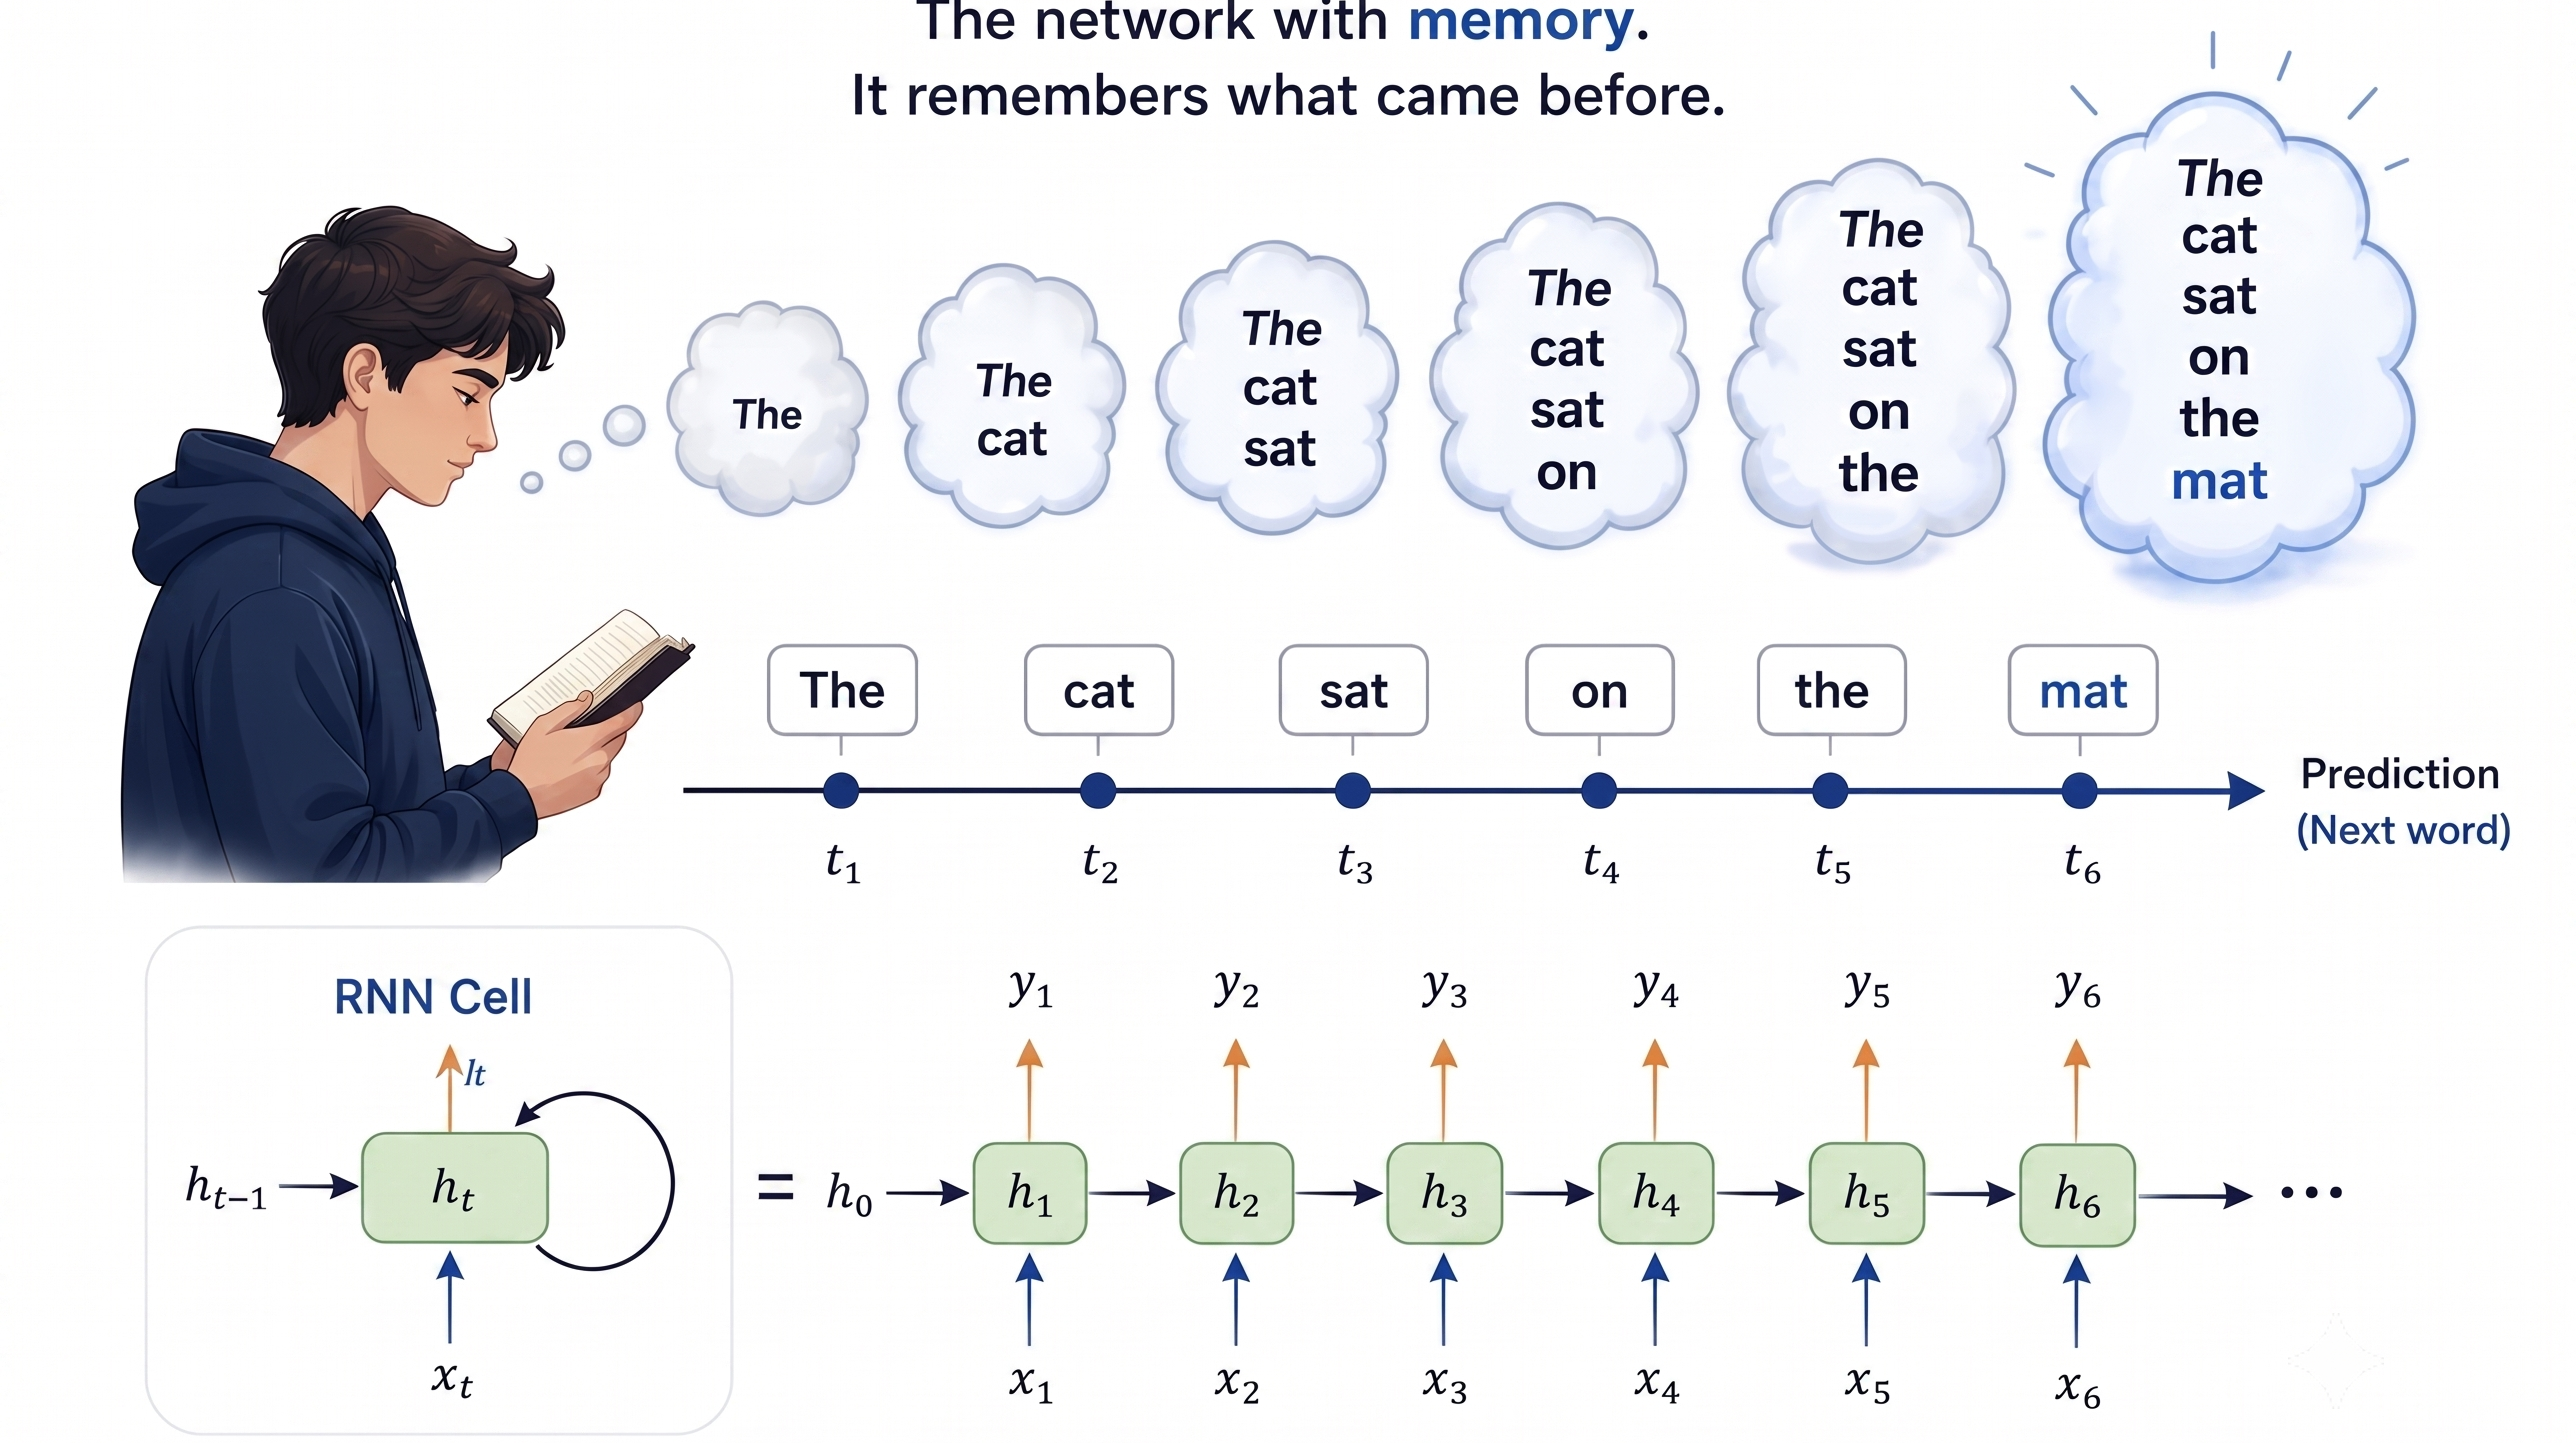
\includegraphics[width=0.95\textwidth]{figures/rnn.png}
\end{figure}
At each time step $t$, the output $y_t$ is computed from hidden state $h_t$:

\begin{equation}
y_t = g(W_{hy} h_t + b_y)
\end{equation}
where $g$ is the output activation function ($g \in \{\text{sigmoid}, \text{softmax}, \text{linear}\}$).

\begin{propertybox}[Parameter Sharing Across Time Steps]
The weight matrices $W_{hh}, W_{xh}$, and $W_{hy}$ are \textbf{shared across all time steps}. The exact same parameters process the transition between $x_1 \to h_1, x_2 \to h_2$, and $x_3 \to h_3$.
\end{propertybox}

\begin{figure}[htbp]
\centering
\begin{tikzpicture}[node distance=2.2cm, >=stealth, auto]
    % Initial state h0
    \node[circle, draw=primaryblue, fill=lightbg, thick, minimum size=0.9cm] (h0) {$h_0$};
    
    % Hidden states h1, h2, h3
    \node[circle, draw=primaryblue, fill=lightbg, thick, minimum size=0.9cm, right of=h0] (h1) {$h_1$};
    \node[circle, draw=primaryblue, fill=lightbg, thick, minimum size=0.9cm, right of=h1] (h2) {$h_2$};
    \node[circle, draw=primaryblue, fill=lightbg, thick, minimum size=0.9cm, right of=h2] (h3) {$h_3$};
    
    % Inputs x1, x2, x3
    \node[circle, draw=primaryblue, fill=lightbg, thick, minimum size=0.9cm, below of=h1, node distance=1.8cm] (x1) {$x_1$};
    \node[circle, draw=primaryblue, fill=lightbg, thick, minimum size=0.9cm, below of=h2, node distance=1.8cm] (x2) {$x_2$};
    \node[circle, draw=primaryblue, fill=lightbg, thick, minimum size=0.9cm, below of=h3, node distance=1.8cm] (x3) {$x_3$};
    
    % Outputs y1, y2, y3
    \node[circle, draw=primaryblue, fill=lightbg, thick, minimum size=0.9cm, above of=h1, node distance=1.8cm] (y1) {$y_1$};
    \node[circle, draw=primaryblue, fill=lightbg, thick, minimum size=0.9cm, above of=h2, node distance=1.8cm] (y2) {$y_2$};
    \node[circle, draw=primaryblue, fill=lightbg, thick, minimum size=0.9cm, above of=h3, node distance=1.8cm] (y3) {$y_3$};
    
    % Labels for inputs and outputs
    \node[below=0.15cm of x1, font=\small] {input at $t=1$};
    \node[below=0.15cm of x2, font=\small] {input at $t=2$};
    \node[below=0.15cm of x3, font=\small] {input at $t=3$};
    
    \node[above=0.15cm of y1, font=\small] {output at $t=1$};
    \node[above=0.15cm of y2, font=\small] {output at $t=2$};
    \node[above=0.15cm of y3, font=\small] {output at $t=3$};
    
    % Input arrows
    \draw[->, thick, primaryblue] (x1) -- (h1) node[midway, right] {$W_{xh}$};
    \draw[->, thick, primaryblue] (x2) -- (h2) node[midway, right] {$W_{xh}$};
    \draw[->, thick, primaryblue] (x3) -- (h3) node[midway, right] {$W_{xh}$};
    
    % Recurrent arrows
    \draw[->, very thick, secondaryblue] (h0) -- (h1) node[midway, above] {$W_{hh}$};
    \draw[->, very thick, secondaryblue] (h1) -- (h2) node[midway, above] {$W_{hh}$};
    \draw[->, very thick, secondaryblue] (h2) -- (h3) node[midway, above] {$W_{hh}$};
    
    % Output arrows
    \draw[->, thick, primaryblue] (h1) -- (y1) node[midway, right] {$W_{hy}$};
    \draw[->, thick, primaryblue] (h2) -- (y2) node[midway, right] {$W_{hy}$};
    \draw[->, thick, primaryblue] (h3) -- (y3) node[midway, right] {$W_{hy}$};
\end{tikzpicture}
\caption{Unrolled Simple Recurrent Neural Network Computational Graph (Page 56).}
\label{fig:simple_rnn_unrolled_custom}
\end{figure}

\section{Sequence Topologies \& Encoder-Decoder Models}

Recurrent neural networks flex to match different task structures, as categorized by Andrej Karpathy:

\begin{enumerate}
    \item \textbf{One-to-One:} Standard fixed input to fixed output ($y = f(x)$).
    \item \textbf{One-to-Many:} Single input produces sequence output (e.g., Image Captioning, Music Generation).
    \item \textbf{Many-to-One:} Sequence input produces single output (e.g., Sentiment Analysis, Text Classification).
    \item \textbf{Many-to-Many (Synchronized):} Sequence input produces synchronized sequence output of same length $T$ (e.g., Video Frame Labeling, POS Tagging).
    \item \textbf{Many-to-Many (Asynchronous / Encoder-Decoder):} Sequence input of length $T_x$ produces sequence output of length $T_y$ (e.g., Machine Translation).
\end{enumerate}

\begin{figure}[htbp]
\centering
\begin{tikzpicture}[scale=0.82, transform shape, >=stealth]
    % 1-to-1
    \node[draw=primaryblue, fill=lightbg, circle] (x11) at (0,0) {$x$};
    \node[draw=primaryblue, fill=lightbg, circle] (h11) at (0,1.5) {$h$};
    \node[draw=primaryblue, fill=lightbg, circle] (y11) at (0,3.0) {$y$};
    \draw[->, thick] (x11)--(h11); \draw[->, thick] (h11)--(y11);
    \node at (0,-0.8) {\textbf{One-to-One}};

    % 1-to-Many
    \node[draw=primaryblue, fill=lightbg, circle] (x21) at (3,0) {$x$};
    \node[draw=primaryblue, fill=lightbg, circle] (h21) at (3,1.5) {$h_1$};
    \node[draw=primaryblue, fill=lightbg, circle] (h22) at (4.2,1.5) {$h_2$};
    \node[draw=primaryblue, fill=lightbg, circle] (y21) at (3,3.0) {$y_1$};
    \node[draw=primaryblue, fill=lightbg, circle] (y22) at (4.2,3.0) {$y_2$};
    \draw[->, thick] (x21)--(h21); \draw[->, thick] (h21)--(h22);
    \draw[->, thick] (h21)--(y21); \draw[->, thick] (h22)--(y22);
    \node at (3.6,-0.8) {\textbf{One-to-Many}};

    % Many-to-1
    \node[draw=primaryblue, fill=lightbg, circle] (x31) at (7,0) {$x_1$};
    \node[draw=primaryblue, fill=lightbg, circle] (x32) at (8.2,0) {$x_2$};
    \node[draw=primaryblue, fill=lightbg, circle] (h31) at (7,1.5) {$h_1$};
    \node[draw=primaryblue, fill=lightbg, circle] (h32) at (8.2,1.5) {$h_2$};
    \node[draw=primaryblue, fill=lightbg, circle] (y32) at (8.2,3.0) {$y$};
    \draw[->, thick] (x31)--(h31); \draw[->, thick] (x32)--(h32);
    \draw[->, thick] (h31)--(h32); \draw[->, thick] (h32)--(y32);
    \node at (7.6,-0.8) {\textbf{Many-to-One}};

    % Many-to-Many Sync
    \node[draw=primaryblue, fill=lightbg, circle] (x41) at (11,0) {$x_1$};
    \node[draw=primaryblue, fill=lightbg, circle] (x42) at (12.2,0) {$x_2$};
    \node[draw=primaryblue, fill=lightbg, circle] (h41) at (11,1.5) {$h_1$};
    \node[draw=primaryblue, fill=lightbg, circle] (h42) at (12.2,1.5) {$h_2$};
    \node[draw=primaryblue, fill=lightbg, circle] (y41) at (11,3.0) {$y_1$};
    \node[draw=primaryblue, fill=lightbg, circle] (y42) at (12.2,3.0) {$y_2$};
    \draw[->, thick] (x41)--(h41); \draw[->, thick] (x42)--(h42);
    \draw[->, thick] (h41)--(h42);
    \draw[->, thick] (h41)--(y41); \draw[->, thick] (h42)--(y42);
    \node at (11.6,-0.8) {\textbf{Many-to-Many (Sync)}};
\end{tikzpicture}
\caption{RNN Sequence Topologies (Karpathy).}
\label{fig:topologies_ch3}
\end{figure}
\clearpage
\section{Backpropagation Through Time (BPTT)}

Backpropagation Through Time (BPTT) extends standard backpropagation by unrolling the recurrent network through time and computing gradients across all time steps.

\begin{figure}[htbp]
\centering
\begin{tikzpicture}[node distance=1.8cm, >=stealth, auto,
    state/.style={circle, draw=primaryblue, fill=lightbg, thick, minimum size=1.0cm},
    arrow/.style={->, thick, primaryblue},
    recarrow/.style={->, very thick, secondaryblue}
]
    % Left side: Folded view
    \node[state] (h_folded) {$h$};
    \node[below=1.2cm of h_folded] (x_folded) {$x$};
    \node[above=1.2cm of h_folded] (z_folded) {$z$};
    
    \draw[arrow] (x_folded) -- (h_folded) node[midway, left] {$W_{xh}$};
    \draw[arrow] (h_folded) -- (z_folded) node[midway, left] {$W_{zh}$};
    \draw[recarrow] (h_folded.east) arc (-90:180:0.45cm) node[midway, right] {$W_{hh}$} (h_folded.north);
    
    % Unfolding Arrow
    \node[right=1.2cm of h_folded, align=center] (unfold) {\Large $\Longrightarrow$\\[0.2em] \small \textbf{Unfolding}};
    
    % Right side: Unrolled view
    \node[state, right=1.6cm of unfold] (h_t1) {$h_{t-1}$};
    \node[state, right=1.8cm of h_t1] (h_t) {$h_t$};
    \node[state, right=1.8cm of h_t] (h_t2) {$h_{t+1}$};
    \node[right=0.8cm of h_t2] (dots) {};
    
    \node[below=1.2cm of h_t1] (x_t1) {$x_{t-1}$};
    \node[below=1.2cm of h_t] (x_t) {$x_t$};
    \node[below=1.2cm of h_t2] (x_t2) {$x_{t+1}$};
    
    \node[above=1.2cm of h_t1] (z_t1) {$z^{(t-1)}$};
    \node[above=1.2cm of h_t] (z_t) {$z^{(t)}$};
    \node[above=1.2cm of h_t2] (z_t2) {$z^{(t+1)}$};
    
    \draw[arrow] (x_t1) -- (h_t1); \draw[arrow] (x_t) -- (h_t); \draw[arrow] (x_t2) -- (h_t2);
    \draw[arrow] (h_t1) -- (z_t1); \draw[arrow] (h_t) -- (z_t); \draw[arrow] (h_t2) -- (z_t2);
    \draw[recarrow] (h_t1) -- (h_t); \draw[recarrow] (h_t) -- (h_t2); \draw[recarrow] (h_t2) -- (dots);
\end{tikzpicture}
\caption{Backpropagation Through Time (BPTT) Unrolled Graph.}
\label{fig:bptt_diagram_custom}
\end{figure}
\clearpage
\section{Long Short-Term Memory (LSTM)}

\textbf{LSTM:}

The Long Short-Term Memory (LSTM) network was proposed in 1997. Its objectives are to:
\begin{itemize}
    \item Preserve information over long sequences.
    \item Reduce the vanishing-gradient problem.
    \item Learn both short-term and long-term dependencies.
    \item Decide automatically which information to keep or discard.
\end{itemize}

Unlike a simple RNN, an LSTM has two states:
\begin{itemize}
    \item \textbf{Hidden state $h_t$:} The short-term memory used to produce outputs.
    \item \textbf{Cell state $C_t$:} The long-term memory that carries information through the sequence.
\end{itemize}

\begin{propertybox}[Key Concept]
The cell state carries the LSTM's key information.
\end{propertybox}

\begin{figure}[htbp]
\centering
\includegraphics[width=0.95\textwidth]{3-RNN/lstm_cell.png}
\caption{Detailed Long Short-Term Memory (LSTM) Cell Architecture.}
\label{fig:lstm_cell_detailed_custom}
\end{figure}

\subsection{Cell State}

\textbf{Cell state:} A vector denoted by $C_t$ that stores long-term information across time steps. Unlike the hidden state, the cell state is designed to let information flow through many time steps with only small modifications. Often described as a ``memory highway,'' it is updated gradually from $C_{t-1}$ to $C_t$ rather than being completely recomputed at every step.

The gates decide how much information is forgotten, added, or exposed.

\begin{advbox}[Intuition]
Imagine reading a book:
\begin{itemize}
    \item You remember the main story (cell state)
    \item You temporarily focus on the current sentence (hidden state)
\end{itemize}
The cell state acts like long-term memory, while the hidden state represents the current understanding.
\end{advbox}

\subsection{LSTM Gates}

An LSTM contains three gates:
\begin{enumerate}
    \item Forget gate
    \item Input gate
    \item Output gate
\end{enumerate}

Each gate is implemented using the sigmoid activation function $\sigma(x) = \frac{1}{1 + e^{-x}}$, where $0 \le \sigma(x) \le 1$.
\begin{itemize}
    \item \textbf{0:} completely block the information
    \item \textbf{1:} pass all the information
    \item \textbf{intermediate values $\to$} partially pass information
\end{itemize}
The gates behave like intelligent switches.

\subsubsection{I) Forget Gate}

The forget gate determines which information from the previous cell state should be retained. It computes:
\begin{equation}
f_t = \sigma(W_f [h_{t-1}, x_t] + b_f)
\end{equation}
where:
\begin{itemize}
    \item $W_f$: forget-gate weight matrix
    \item $b_f$: forget-gate bias
    \item $[h_{t-1}, x_t]$: concatenation of the previous hidden state and current input.
\end{itemize}

\begin{itemize}
    \item If $f_t = 1$, the previous memory is fully preserved.
    \item If $f_t = 0$, the previous memory is completely erased.
    \item If $f_t = 0.4$, 40\% is retained.
\end{itemize}

\subsubsection{II) Input Gate}

The input gate determines which new information should be stored. It has two parts:
\begin{enumerate}
    \item \textbf{Gate Activation:} $i_t = \sigma(W_i [h_{t-1}, x_t] + b_i)$
    \item \textbf{Candidate Memory:} $\tilde{C}_t = \tanh(W_c [h_{t-1}, x_t] + b_c)$
\end{enumerate}

The candidate memory contains the new information that may be written into the cell state.

\begin{propertybox}[Input Gate Example]
Example $i_t = \begin{bmatrix} 1 \\ 0.3 \end{bmatrix}$ and $\tilde{C}_t = \begin{bmatrix} 2 \\ 5 \end{bmatrix}$ then $i_t \otimes \tilde{C}_t = \begin{bmatrix} 2 \\ 1.5 \end{bmatrix}$.\\
Only a fraction of the second candidate value is stored.
\end{propertybox}

\subsubsection{III) Output Gate}

The output gate determines which information from the cell state becomes the hidden state.
\begin{align}
\text{First: } & o_t = \sigma(W_o [h_{t-1}, x_t] + b_o) \\
\text{Then: } & h_t = o_t \otimes \tanh(C_t)
\end{align}

The hidden state $h_t$ is:
\begin{itemize}
    \item passed to the next LSTM cell
    \item used to compute the next network's output.
\end{itemize}

\subsubsection{IV) Cell State Update}

The cell state is updated by combining the retained old memory with the selected new memory:
\begin{equation}
C_t = f_t \otimes C_{t-1} + i_t \otimes \tilde{C}_t
\end{equation}
This is the central equation of the LSTM.

\begin{propertybox}[Complete Forward Pass]
\begin{align}
f_t &= \sigma(W_f [h_{t-1}, x_t] + b_f) \\
i_t &= \sigma(W_i [h_{t-1}, x_t] + b_i) \\
\tilde{C}_t &= \tanh(W_c [h_{t-1}, x_t] + b_c) \\
C_t &= f_t \otimes C_{t-1} + i_t \otimes \tilde{C}_t \\
o_t &= \sigma(W_o [h_{t-1}, x_t] + b_o) \\
h_t &= o_t \otimes \tanh(C_t)
\end{align}
These six equations define a standard LSTM cell.
\end{propertybox}

\subsection{Complexity \& Why LSTM Works}

\textbf{Complexity:} Four matrix multiplications
\begin{equation}
\mathcal{O}(4(n_x n_h + n_h^2)) \sim \mathcal{O}(n_x n_h + n_h^2)
\end{equation}
For a sequence of length $T$:
\begin{equation}
\mathcal{O}(T(n_x n_h + n_h^2))
\end{equation}
Compared with a simple RNN, an LSTM is roughly four times more expensive per time step because it computes four gates instead of one hidden-state update.

\textbf{LSTMs work because:}
\begin{itemize}
    \item \textbf{The forget gate:} removes irrelevant information
    \item \textbf{The input gate:} writes useful new information
    \item \textbf{The output gate:} decides what information should influence the current prediction
\end{itemize}
Because the cell-state update contains an additive term $C_t = f_t \otimes C_{t-1} + i_t \otimes \tilde{C}_t$, gradients can propagate through many time steps more effectively than in a simple RNN, greatly reducing the vanishing-gradient problem. Although LSTMs do not completely eliminate gradient issues, they are better able to learn long-range dependencies.

\subsection{Advantages \& Limitations}

\begin{advbox}[Advantages]
\begin{itemize}
    \item Captures long-term dependencies
    \item Greatly reduces the vanishing gradient problem
    \item Learns which information to remember and which to forget
    \item Performs well on NLP, speech recognition, and machine translation
    \item Supports variable-length input sequences
\end{itemize}
\end{advbox}

\begin{advbox}[Limitations]
\begin{itemize}
    \item More parameters than a simple RNN, increasing memory requirements
    \item Higher computational cost due to the four gates
    \item Longer training times
    \item More difficult to interpret because multiple gates interact simultaneously
\end{itemize}
\end{advbox}

\section{Gated Recurrent Unit (GRU)}

\textbf{Introduction:} The GRU is a recurrent neural network architecture introduced in 2014 as a simplified alternative to the LSTM.

\textbf{The main objectives of the GRU are to:}
\begin{itemize}
    \item Learn long-term dependencies
    \item Reduce the vanishing gradient problem
    \item Simplify the LSTM architecture
    \item Reduce the number of trainable parameters
    \item Train faster while achieving comparable performance.
\end{itemize}

\textbf{The GRU simplifies the LSTM architecture by:}
\begin{itemize}
    \item Removing the separate cell state
    \item Combining forget and input mechanisms into a single update gate
    \item Keeping only one memory vector: the hidden state.
\end{itemize}

\textbf{The GRU balances simplicity and performance.}

\begin{figure}[htbp]
\centering
\includegraphics[width=0.95\textwidth]{3-RNN/gru_cell.png}
\caption{Conceptual overview of the Gated Recurrent Unit (GRU): one hidden state is selectively reset and blended at each time step.}
\label{fig:gru_architecture_custom_p74}
\end{figure}

\subsection{Update Gate \& Reset Gate}

\subsubsection{II) Update Gate}

The update gate determines how much of the previous hidden state should be retained. It plays a role similar to the combined action of the forget and input gates in an LSTM:
\begin{equation}
z_t = \sigma(W_z x_t + U_z h_{t-1} + b_z) \quad \text{where }
\begin{cases}
W_z: \text{input weights} \\
U_z: \text{recurrent weights} \\
b_z: \text{bias}
\end{cases}, \quad 0 \le z_t \le 1
\end{equation}

The gate controls the proportion of old versus new information:
\begin{itemize}
    \item $z_t = 1$: the previous hidden state is almost preserved
    \item $z_t = 0$: the model ignores the previous state and relies on newly computed information
\end{itemize}

\subsubsection{III) Reset Gate}

The reset gate determines how much of the previous memory should be ignored when computing the new candidate hidden state:
\begin{equation}
r_t = \sigma(W_r x_t + U_r h_{t-1} + b_r)
\end{equation}
\begin{itemize}
    \item $r_t = 0$: the previous hidden state is almost completely ignored
    \item $r_t = 1$: all previous information is considered
\end{itemize}
It is useful when the model needs to discard outdated context and start processing a new pattern.

\subsection{Candidate Hidden State \& Forward Pass}

\textbf{Candidate Hidden State:}
\begin{equation}
\tilde{h}_t = \tanh(W_h x_t + U_h (r_t \otimes h_{t-1}) + b_h)
\end{equation}

The new hidden state is obtained by combining:
\begin{itemize}
    \item the previous hidden state
    \item the candidate hidden state
\end{itemize}

\begin{propertybox}[Complete Forward Pass]
\begin{align}
\text{Update Gate: } & z_t = \sigma(W_z x_t + U_z h_{t-1} + b_z) \\
\text{Reset Gate: } & r_t = \sigma(W_r x_t + U_r h_{t-1} + b_r) \\
\text{Candidate Hidden State: } & \tilde{h}_t = \tanh(W_h x_t + U_h (r_t \otimes h_{t-1}) + b_h) \\
\text{Hidden State: } & h_t = z_t \otimes h_{t-1} + (1 - z_t) \otimes \tilde{h}_t
\end{align}
These four equations completely define the GRU.
\end{propertybox}

\begin{figure}[htbp]
\centering
\begin{tikzpicture}[node distance=1.4cm, >=stealth, auto, scale=0.92, transform shape,
    box/.style={rectangle, draw=primaryblue, fill=blue!10, thick, rounded corners=5pt, minimum width=3.8cm, minimum height=0.9cm, align=center},
    gatebox/.style={rectangle, draw=accentred, fill=red!10, thick, rounded corners=5pt, minimum width=3.2cm, minimum height=0.9cm, align=center},
    opbox/.style={rectangle, draw=secondaryblue, fill=teal!10, thick, rounded corners=5pt, minimum width=3.8cm, minimum height=0.9cm, align=center},
    eqbox/.style={rectangle, draw=primaryblue, fill=boxbg, double, thick, rounded corners=5pt, minimum width=6.2cm, minimum height=1.0cm, align=center}
]
    % Top center node
    \node[box] (hprev) at (0, 4.2) {\textbf{Previous Hidden State $h_{t-1}$}};

    % Symmetric Gate branches
    \node[gatebox] (update) at (-3.4, 2.6) {\textbf{Update Gate $z_t$}};
    \node[gatebox] (reset) at (3.4, 2.6) {\textbf{Reset Gate $r_t$}};

    % Under reset gate
    \node[opbox] (reset_state) at (3.4, 1.2) {$r_t \otimes h_{t-1}$};
    \node[opbox] (candidate) at (3.4, -0.2) {\textbf{Candidate Hidden State $\tilde{h}_t$}};

    % Centered Combination equation box
    \node[eqbox] (combine) at (0, -1.8) {$h_t = z_t \otimes h_{t-1} + (1 - z_t) \otimes \tilde{h}_t$};

    % Bottom center node
    \node[box] (hnew) at (0, -3.2) {\textbf{New Hidden State $h_t$}};

    % Symmetric Connecting Arrows
    \draw[->, thick, primaryblue] (hprev.south) -| (update.north);
    \draw[->, thick, primaryblue] (hprev.south) -| (reset.north);
    \draw[->, thick, accentred] (reset.south) -- (reset_state.north);
    \draw[->, thick, secondaryblue] (reset_state.south) -- (candidate.north);
    \draw[->, thick, primaryblue] (update.south) |- (combine.west);
    \draw[->, thick, secondaryblue] (candidate.south) |- (combine.east);
    \draw[->, thick, primaryblue] (combine.south) -- (hnew.north);
\end{tikzpicture}
\caption{GRU Computational Graph Flowchart.}
\label{fig:gru_computational_graph_p77}
\end{figure}

\subsection{Complexity, Why GRU Works, Advantages \& Limitations}

\textbf{Complexity:} $\mathcal{O}(T(n_x n_h + n_h^2))$

The GRU performs fewer matrix multiplications because it has only three parameter groups instead of four.

\textbf{Why GRU works:}
The GRU is effective because it uses gating mechanisms to regulate the flow of information without requiring a separate cell state. The update gate controls how much past information is preserved, while the reset gate determines how much past information influences the candidate hidden state.

The network can preserve information across many time steps when needed, allowing gradients to propagate more effectively than in a simple RNN. Although GRUs do not eliminate vanishing gradients entirely, they substantially mitigate the problem while remaining computationally efficient.

\begin{advbox}[Advantages]
\begin{itemize}
    \item Simpler than LSTM
    \item Faster training
    \item Lower memory consumption
    \item Excellent performance on many NLP tasks
    \item Easier to optimize due to its simpler architecture
\end{itemize}
\end{advbox}

\begin{advbox}[Limitations]
\begin{itemize}
    \item Slightly less expressive than an LSTM because it lacks a separate cell state
    \item Performance can be task-dependent; some applications benefit more from the additional flexibility of LSTMs.
    \item Like other recurrent models, GRUs process sequences sequentially, which limits parallelization compared with Transformer architectures.
\end{itemize}
\end{advbox}

The GRU offers a compelling compromise between the simplicity of a simple RNN and the expressive power of an LSTM, making it a widely used architecture for many real-world sequence-modeling tasks.

\section{Deep (Stacked) Recurrent Neural Networks}

\textbf{I) Stacked (Deep) RNNs}

The motivation for using stacked RNNs (also known as Deep RNNs) is to increase the model's capacity to learn more abstract, hierarchical representations of sequential data, which a single-layer RNN may fail to capture.
\begin{itemize}
    \item \textbf{Lower layer:} can focus on extracting simpler temporal patterns or local features from the raw input sequences.
    \item \textbf{Higher layer:} build upon these extracted features to learn more complex, long-range dependencies, making the overall model more powerful.
\end{itemize}

\begin{figure}[htbp]
\centering
\begin{tikzpicture}[node distance=1.6cm, >=stealth, auto, scale=0.92, transform shape]
    % Output layer
    \node[rectangle, draw=purple, fill=purple!10, thick, rounded corners=3pt] (o1) at (0, 4.5) {$O_{t-1}$};
    \node[rectangle, draw=purple, fill=purple!10, thick, rounded corners=3pt] (o2) at (3, 4.5) {$O_t$};
    \node[rectangle, draw=purple, fill=purple!10, thick, rounded corners=3pt] (o3) at (6, 4.5) {$O_{t+1}$};
    
    \node[rectangle, draw=primaryblue, fill=lightbg, thick] (y1) at (0, 5.7) {$Y_{t-1}$};
    \node[rectangle, draw=primaryblue, fill=lightbg, thick] (y2) at (3, 5.7) {$Y_t$};
    \node[rectangle, draw=primaryblue, fill=lightbg, thick] (y3) at (6, 5.7) {$Y_{t+1}$};
    
    % Layer L (top layer)
    \node[rectangle, draw=teal, fill=teal!10, thick, rounded corners=3pt] (hL1) at (0, 3.2) {$h_{t-1}^{(L)}$};
    \node[rectangle, draw=teal, fill=teal!10, thick, rounded corners=3pt] (hL2) at (3, 3.2) {$h_t^{(L)}$};
    \node[rectangle, draw=teal, fill=teal!10, thick, rounded corners=3pt] (hL3) at (6, 3.2) {$h_{t+1}^{(L)}$};
    
    % Layer 1 (bottom layer)
    \node[rectangle, draw=teal, fill=teal!10, thick, rounded corners=3pt] (h11) at (0, 1.6) {$h_{t-1}^{(1)}$};
    \node[rectangle, draw=teal, fill=teal!10, thick, rounded corners=3pt] (h12) at (3, 1.6) {$h_t^{(1)}$};
    \node[rectangle, draw=teal, fill=teal!10, thick, rounded corners=3pt] (h13) at (6, 1.6) {$h_{t+1}^{(1)}$};
    
    % Input layer
    \node[rectangle, draw=primaryblue, fill=blue!10, thick] (x1) at (0, 0) {$x_{t-1}$};
    \node[rectangle, draw=primaryblue, fill=blue!10, thick] (x2) at (3, 0) {$x_t$};
    \node[rectangle, draw=primaryblue, fill=blue!10, thick] (x3) at (6, 0) {$x_{t+1}$};
    
    % Horizontal recurrent connections
    \draw[->, thick, primaryblue] (h11) -- (h12); \draw[->, thick, primaryblue] (h12) -- (h13);
    \draw[->, thick, primaryblue] (hL1) -- (hL2); \draw[->, thick, primaryblue] (hL2) -- (hL3);
    
    % Vertical connections between layers
    \draw[->, thick] (x1) -- (h11); \draw[->, thick] (x2) -- (h12); \draw[->, thick] (x3) -- (h13);
    \draw[->, thick, dashed] (h11) -- (hL1); \draw[->, thick, dashed] (h12) -- (hL2); \draw[->, thick, dashed] (h13) -- (hL3);
    \draw[->, thick] (hL1) -- (o1); \draw[->, thick] (hL2) -- (o2); \draw[->, thick] (hL3) -- (o3);
    \draw[->, thick] (o1) -- (y1); \draw[->, thick] (o2) -- (y2); \draw[->, thick] (o3) -- (y3);

    \node[left=0.5cm of h11] {\small Layer 1 (bottom)};
    \node[left=0.5cm of hL1] {\small Layer $L$ (top)};
    \node[left=0.5cm of o1] {\small Output layer};
\end{tikzpicture}
\caption{Stacked (Deep) Recurrent Neural Network Architecture.}
\label{fig:stacked_rnn_p81}
\end{figure}

Stacking recurrent layers increases the capacity of the per-step transformation while keeping temporal recursion at every level. This tends to help when the dataset is large enough to support more parameters without overfitting, a bias-variance trade-off that also applies to depth in any network.

Each layer has its own independent set of weights; nothing is shared across layers.

\textbf{Implementation:}
\begin{lstlisting}[language=Python]
model.add(LSTM(state_dim, return_sequences=True))
model.add(LSTM(state_dim, return_sequences=True))
model.add(LSTM(state_dim, return_sequences=True))
model.add(Dense(1, activation='sigmoid'))
\end{lstlisting}

\textbf{General Equation:}
\begin{equation}
h_t^{(l)} = f(W^{(l)} h_t^{(l-1)} + U^{(l)} h_{t-1}^{(l)} + b^{(l)})
\end{equation}

Stacked RNN are more prone to overfitting.
\textbf{Dropout randomly:} The Goal is to improve generalization without changing the architecture.

\section{Bidirectional Recurrent Neural Networks (Bi-RNN)}

\textbf{II) Bidirectional RNNs (Bi-RNN)}

\begin{figure}[htbp]
\centering
\begin{tikzpicture}[scale=0.9, transform shape, >=stealth]
    % Output Row
    \node[rectangle, draw=darkslate, fill=white, thick, minimum size=0.8cm] (o1) at (0, 4.5) {$O_1$};
    \node[rectangle, draw=darkslate, fill=white, thick, minimum size=0.8cm] (o2) at (2.5, 4.5) {$O_2$};
    \node[rectangle, draw=darkslate, fill=white, thick, minimum size=0.8cm] (o3) at (5.0, 4.5) {$O_3$};
    \node[rectangle, draw=darkslate, fill=white, thick, minimum size=0.8cm] (oT) at (7.5, 4.5) {$O_T$};
    
    % Forward Hidden Row (Green)
    \node[rectangle, draw=teal, fill=teal!15, thick, minimum size=0.8cm] (f1) at (0, 3.0) {$\overrightarrow{H}_1$};
    \node[rectangle, draw=teal, fill=teal!15, thick, minimum size=0.8cm] (f2) at (2.5, 3.0) {$\overrightarrow{H}_2$};
    \node[rectangle, draw=teal, fill=teal!15, thick, minimum size=0.8cm] (f3) at (5.0, 3.0) {$\overrightarrow{H}_3$};
    \node[rectangle, draw=teal, fill=teal!15, thick, minimum size=0.8cm] (fT) at (7.5, 3.0) {$\overrightarrow{H}_T$};
    
    % Backward Hidden Row (Red)
    \node[rectangle, draw=accentred, fill=red!10, thick, minimum size=0.8cm] (b1) at (0, 1.5) {$\overleftarrow{H}_1$};
    \node[rectangle, draw=accentred, fill=red!10, thick, minimum size=0.8cm] (b2) at (2.5, 1.5) {$\overleftarrow{H}_2$};
    \node[rectangle, draw=accentred, fill=red!10, thick, minimum size=0.8cm] (b3) at (5.0, 1.5) {$\overleftarrow{H}_3$};
    \node[rectangle, draw=accentred, fill=red!10, thick, minimum size=0.8cm] (bT) at (7.5, 1.5) {$\overleftarrow{H}_T$};
    
    % Input Row (Blue)
    \node[rectangle, draw=primaryblue, fill=blue!10, thick, minimum size=0.8cm] (x1) at (0, 0) {$X_1$};
    \node[rectangle, draw=primaryblue, fill=blue!10, thick, minimum size=0.8cm] (x2) at (2.5, 0) {$X_2$};
    \node[rectangle, draw=primaryblue, fill=blue!10, thick, minimum size=0.8cm] (x3) at (5.0, 0) {$X_3$};
    \node[rectangle, draw=primaryblue, fill=blue!10, thick, minimum size=0.8cm] (xT) at (7.5, 0) {$X_T$};
    
    % Forward Horizontal Connections (Green)
    \draw[->, thick, teal] (f1) -- (f2); \draw[->, thick, teal] (f2) -- (f3);
    \draw[->, thick, teal] (f3) -- node[midway, fill=white] {$\dots$} (fT);
    
    % Backward Horizontal Connections (Red)
    \draw[->, thick, accentred] (bT) -- node[midway, fill=white] {$\dots$} (b3);
    \draw[->, thick, accentred] (b3) -- (b2); \draw[->, thick, accentred] (b2) -- (b1);
    
    % Inputs to Hidden
    \draw[->, thick] (x1) -- (b1); \draw[->, thick] (x2) -- (b2); \draw[->, thick] (x3) -- (b3); \draw[->, thick] (xT) -- (bT);
    \draw[->, thick, teal, bend left=30] (x1) to (f1);
    \draw[->, thick, teal, bend left=30] (x2) to (f2);
    \draw[->, thick, teal, bend left=30] (x3) to (f3);
    \draw[->, thick, teal, bend left=30] (xT) to (fT);
    
    % Hidden to Output
    \draw[->, thick] (f1) -- (o1); \draw[->, thick] (f2) -- (o2); \draw[->, thick] (f3) -- (o3); \draw[->, thick] (fT) -- (oT);
    \draw[->, thick, accentred, bend right=30] (b1) to (o1);
    \draw[->, thick, accentred, bend right=30] (b2) to (o2);
    \draw[->, thick, accentred, bend right=30] (b3) to (o3);
    \draw[->, thick, accentred, bend right=30] (bT) to (oT);
\end{tikzpicture}
\caption{Bidirectional Recurrent Neural Network (Bi-RNN) Graph.}
\label{fig:birnn_p83}
\end{figure}

\textbf{Motivation:}
Many machine learning problems require understanding both past and Future context.

\begin{advbox}[Context Example]
\begin{align*}
\text{Example: } & \text{I deposited money in the bank} \to \text{Financial institution} \\
& \text{The Fisherman sat on the bank} \to \text{river Bank}
\end{align*}
So The: Previous words are insufficient. Future words are also important.
Understanding both left and Right Contexts improves interpretation.
\end{advbox}

Instead of One recurrent network we build two independent RNN:
\begin{itemize}
    \item \textbf{One Process:} Left $\to$ Right
    \item \textbf{The Second:} Left $\gets$ Right
\end{itemize}
Both networks analyze the same sentence independently. Finally, their outputs are merged.

\begin{align}
\text{Forward Hidden State: } & \overrightarrow{h}_t = \phi(W_f x_t + U_f \overrightarrow{h}_{t-1} + b_f) \\
\text{Backward Hidden State: } & \overleftarrow{h}_t = \phi(W_b x_t + U_b \overleftarrow{h}_{t+1} + b_b) \\
\text{The final Representation: } & h_t = [\overrightarrow{h}_t, \overleftarrow{h}_t]
\end{align}

\subsection{Bidirectional LSTM (Bi-LSTM)}

Instead of Using two Simple RNNs we Can Use two LSTM:
\begin{align}
\text{Forward LSTM compute: } & \overrightarrow{h}_t, \overrightarrow{C}_t \\
\text{Backward LSTM Compute: } & \overleftarrow{h}_t, \overleftarrow{C}_t \\
\text{Final output: } & h_t = [\overrightarrow{h}_t; \overleftarrow{h}_t]
\end{align}

Bi-LSTM combine the advantages of:
\begin{itemize}
    \item Long-term memory (LSTM)
    \item Future context (Bidirectional Processing)
\end{itemize}

\subsection{Limitations \& Practical Considerations}

\begin{advbox}[Limitation]
\begin{itemize}
    \item Approximately twice as many RNN parameters
    \item Increased GPU memory Consumption
    \item Long training and inference time
    \item Cannot be used for real time prediction because future inputs are Required.
\end{itemize}
\end{advbox}

\begin{propertybox}[Practical Consideration]
\begin{itemize}
    \item Use Simple RNN only For simple education examples
    \item Use LSTM when Long Term dependencies are important
    \item Use GRU when u need Similar Performance to an LSTM with fewer parameters and Faster training
    \item Use a Bidirectional LSTM when The entire Sequence is available before making a Prediction and Maximum Contextual understanding is Required.
\end{itemize}
\end{propertybox}

\section{Text Generation \& Encoder-Decoder Pipeline}

\textbf{Text Generation with RNN Steps:}

\begin{enumerate}
    \item \textbf{Text Cleaning:}
    \begin{itemize}
        \item Convert all letters to lowercase
        \item Remove unnecessary Symbols
        \item Remove extra Spaces
    \end{itemize}
    \item \textbf{Tokenization:} split text into words to characters
    \item \textbf{Word Indexing:} assign each unique word an integer ID
    \item \textbf{Text to Sequence:} replace words with their Corresponding indices
    \item \textbf{Padding / Truncation:} ensure all Sequences have the Same length for batch processing.
    \item \textbf{Word Embedding:} words are represented as dense vectors instead of one-hot vectors. An Embedding layer transform each word index into a Continuous vector that Captures Semantic relationships. This embedding layer often Contains the Largest number of Parameters in The model.
    \item \textbf{Passed Sentence into RNN Model} that's fast play The Role of Encoder: compressed The entire Sentence into one vector. This vector Summarizes the meaning of The input.
\end{enumerate}

So encoder Produce $h_T$ where $T = \text{last word of The Sentence}$, $h_T = \text{Final hidden State}$.
This hidden state called the: Context Vector OR Sentence Representation.

\begin{enumerate}[resume]
    \item \textbf{Bottleneck (Context Vector):} The encoder passes only one vector to The decoder. This vector is called:
    \begin{itemize}
        \item Context Vector
        \item Latent Vector
        \item Bottleneck
        \item Thought Vector
    \end{itemize}
    The bottleneck contains the information needed to reconstruct or Generate the output Sequence.
    \item \textbf{Decoder:} receives the context vector and Starts Generating the Output Sequence. The decoder Generate one token at time.
\end{enumerate}

\textbf{Decoder Process:}
\begin{enumerate}
    \item Receive the context Vector
    \item Generate one word
    \item Feed the Generated word back into The decoder
    \item Generate the next word
    \item Repeat until End-of-Sequence (EOS) token is produced
\end{enumerate}

\begin{advbox}[Limitation]
\begin{itemize}
    \item Fixed-size bottleneck can be lose information for long Sequence.
    \item Performance decreases as input length increase.
    \item This limitation is addressed by Attention, which allows the decoder to access all encoder hidden states instead of only the final context vector.
\end{itemize}
\end{advbox}

% ====================================================================
% Chapter 3 Continuation: Attention Mechanisms & Image Captioning
% (Digitized directly from Author Manuscript Pages 90 - 105)
% ====================================================================

\section{Attention Mechanism for Seq2Seq RNNs}

The first Seq2Seq (Encoder-Decoder) models solved the problem of mapping an input sequence to an output sequence; however, they suffered from a major limitation: the decoder relied only on a single fixed-size context vector (the bottleneck). For long sentences, this vector could not preserve all the information from the source sequence, causing translation and text generation quality to degrade. 

The \textbf{Attention Mechanism} was introduced to overcome this limitation by allowing the decoder to dynamically focus on the most relevant parts of the input sequence during each decoding step.

\subsection{Main Idea of Attention}

Instead of using only one context vector, the decoder can look at all encoder hidden states whenever it generates a new output word. Instead of $c = h_m$, we compute a different context vector for every decoder step.

So,
\begin{itemize}
    \item Encoder stores all hidden states.
    \item Decoder decides which hidden states are most useful.
    \item The decision is made through attention weights.
\end{itemize}

\begin{figure}[htbp]
\centering
\includegraphics[width=0.92\textwidth]{3-RNN/graph1_seq2seq.png}
\caption{Encoder-Decoder RNN (Seq2Seq) Architecture and Sequence-to-Sequence Performance comparison showing performance degradation without attention versus sustained quality with attention.}
\label{fig:seq2seq_attention_comparison}
\end{figure}

\subsection{Calculate Attention Step by Step}

\begin{itemize}
    \item \textbf{Without attention:} The final state is incapable of remembering a long sequence.
    \item \textbf{With attention:} Seq2Seq model does not forget source input and the decoder knows where to focus.
\end{itemize}

\begin{figure}[htbp]
\centering
\includegraphics[width=0.92\textwidth]{3-RNN/graph2_attention_step_by_step.png}
\caption{Step-by-Step Calculation of Attention: Encoder states $h_i$, Decoder state $S_{t-1}$, Linear Projections, Alignment Score $e_{ti}$, Softmax Attention Weight $\alpha_{ti}$, and Context Vector $c_t$.}
\label{fig:attention_step_by_step_diagram}
\end{figure}

This vector $c_t$ is a focused snapshot of the input sequence; it acts as a dynamic summary that changes for every word the decoder generates.

\textbf{Repeat for every output word:}
Attention is recomputed at every decoder time step:
\begin{enumerate}
    \item Compute alignment
    \item Compute attention weights
    \item Compute context vector $c_t$
\end{enumerate}

\begin{propertybox}[Numerical Example of Attention Weights]
Suppose alignment scores are $e_1 = 1, e_2 = 2, e_3 = 3$.
Applying Softmax normalization:
\begin{equation}
e_1 = \frac{2.7}{30}, \quad e_2 = \frac{7.3}{30}, \quad e_3 = \frac{20}{30}
\end{equation}
resulting in attention weights:
\begin{equation}
\alpha_1 = 0.09, \quad \alpha_2 = 0.20, \quad \alpha_3 = 0.665
\end{equation}
The context vector is computed as:
\begin{equation}
C = \alpha_1 h_1 + \alpha_2 h_2 + \alpha_3 h_3
\end{equation}
Here, state $h_3$ receives the highest weight ($\alpha_3 = 0.665$), receiving the most attention.
\end{propertybox}

\subsection{Advantages \& Limitations of Attention}

\begin{advbox}[Advantages]
\begin{itemize}
    \item Eliminates the fixed-size bottleneck.
    \item Handles long input sequences much better.
    \item Produces better translations and generated text.
    \item Learns where to focus automatically.
    \item Generates a different context vector for each output word.
    \item Greatly improves Seq2Seq performance.
\end{itemize}
\end{advbox}

\begin{advbox}[Limitations]
\begin{itemize}
    \item Higher computational cost.
    \item Increased memory usage.
    \item Attention weights must be recomputed for every decoder step.
    \item Complexity grows with both input and output sequence lengths.
\end{itemize}
\end{advbox}

\begin{propertybox}[Summary of Attention Mechanism]
The Attention Mechanism enhances the classical Encoder-Decoder architecture by allowing the decoder to access all encoder hidden states instead of relying on a single bottleneck vector. At each decoding step, the decoder computes alignment scores, converts them into attention weights using Softmax, forms a context vector as a weighted sum of the encoder hidden states, and uses this context to generate the next output token. Because a new context vector is computed for every output step, the model learns where to focus in the input sequence, greatly improving performance on long sequences at the cost of increased computational complexity.
\end{propertybox}

\section{Self-Attention in RNN}

\textbf{Self-Attention in RNN} is a neural mechanism that enables a model to determine which parts of its own input sequence are the most relevant when computing the representation of the current element. Instead of relying only on the previous hidden state, the model compares the current hidden state with all previous hidden states and selectively focuses on the most informative ones.

In RNNs, self-attention improves the network's ability to model long-range dependencies by allowing it to retrieve information from any previous time step.

\begin{itemize}
    \item \textbf{In Attention:} The decoder looks at the encoder's hidden states.
    \item \textbf{In Self-Attention:} The model looks at previous decoder hidden states, meaning the decoder is attending to its own previous hidden states, in addition to (or instead of) attending to the encoder.
\end{itemize}

\textbf{Decoder Self-Attention:} \textit{"Which words have I already generated that are important for predicting the next word?"}

\textit{Example:} \textit{"Mohamed likes studying at night"} (where \textit{studying} attends back to \textit{Mohamed}).

\begin{figure}[htbp]
\centering
\includegraphics[width=0.88\textwidth]{3-RNN/graph3_decoder.png}
\caption{Decoder architecture integrating self-attention context vectors $C_1, C_2, C_3, C_4$ across hidden states $h_1, h_2, h_3, h_4$.}
\label{fig:decoder_self_attention_graph}
\end{figure}

The updated state and context vectors are formulated as:
\begin{equation}
h_4 = \tanh\left(A \cdot \begin{bmatrix} x_4 \\ C_3 \end{bmatrix} + b\right)
\end{equation}
\begin{equation}
\text{weights: } \alpha_i = \operatorname{align}(h_i, h_4)
\end{equation}
\begin{equation}
C_4 = \alpha_1 h_1 + \alpha_2 h_2 + \alpha_3 h_3 + \alpha_4 h_4 \quad \text{(repeated for every new generated word)}
\end{equation}

\begin{propertybox}[Historical Literature References]
\textbf{Notice:} The original self-attention paper uses LSTM networks. Two foundational papers reference Attention and Self-Attention:
\begin{enumerate}
    \item \textbf{Bahdanau, Cho \& Bengio (2015):} Encoder-Decoder Attention ($\text{Query} = \text{decoder state}$, $\text{Keys}/\text{Values} = \text{encoder states}$ across two different sequences).
    \item \textbf{Cheng, Dong \& Lapata (2016):} \textit{"Long Short-Term Memory Network for Machine Reading"}, where the Query, Keys, and Values all come from the same sequence (a single RNN attending to its own history). This is the direct conceptual ancestor of Transformer self-attention.
\end{enumerate}
\end{propertybox}

\subsection{Self-Attention Mechanism Step-by-Step}

\begin{align}
\tilde{h}_t &= \tanh(A[h_{t-1}, x_t] + b) \\
e_i &= \operatorname{align}(\tilde{h}_t, h_i) \quad \text{for } i = 1, \dots, t \\
e_i &= v^T \tanh(W_1 \tilde{h}_t + W_2 h_i) \\
\alpha_i &= \operatorname{softmax}(e_i) \\
c_t &= \sum_{i=1}^t \alpha_i h_i \quad \text{(context vector, repeat until EOS)}
\end{align}

\begin{advbox}[Advantages of Self-Attention in RNNs]
\begin{itemize}
    \item Reduces forgetting of long-term information.
    \item Allows direct access to earlier hidden states.
    \item Learns automatically where to focus.
    \item Improves the representation of long sequences.
    \item Serves as a bridge between classical RNNs and modern Transformer architectures.
\end{itemize}
\end{advbox}

\begin{advbox}[Limitations of Self-Attention in RNNs]
\begin{itemize}
    \item Computational complexity increases because attention must be computed at every time step.
    \item All hidden states must be stored in memory.
    \item Still processes the sequence sequentially, unlike Transformers which compute self-attention in parallel.
\end{itemize}
\end{advbox}

\section{Image Caption Generation Architecture (CNN-LSTM Model)}

\textbf{Project: Image Caption Generation using CNN and LSTM}

Image Captioning is the task of automatically generating a natural language description for an image. Image captioning combines two major fields:
\begin{itemize}
    \item \textbf{Computer Vision:} to understand the content of the image.
    \item \textbf{Natural Language Processing (NLP):} to generate the describing sentence.
\end{itemize}

\begin{figure}[htbp]
\centering
\includegraphics[width=0.92\textwidth]{3-RNN/graph4_image_captioning.png}
\caption{Complete Image Caption Generation Multimodal System Architecture.}
\label{fig:image_captioning_architecture_multimodal}
\end{figure}

\begin{propertybox}[Dataset: Flickr8K]
\textbf{Characteristics:}
\begin{itemize}
    \item Approximately $8,000$ images.
    \item Every image has $5$ different captions ($30,000$ total captions).
    \item Around $6,000$ images are used for training.
\end{itemize}
\end{propertybox}

\subsection{Pipeline Steps}

\begin{enumerate}
    \item \textbf{Step 1: Feature Extraction (Transfer Learning)} \\
    Instead of training a CNN from scratch (which requires millions of images), the project uses a pretrained VGG16 network via Transfer Learning. The process reuses a model that has already learned rich visual representations from ImageNet.
    
    The final classification layer in VGG16 is removed, leaving a $4096$-dimensional feature vector that summarizes the visual content of the image.

    \item \textbf{Step 2: Captions Processing} \\
    Captions undergo preprocessing:
    \begin{itemize}
        \item Add Special Tokens: \texttt{startseq A child in a pink dress endseq} to indicate start and end boundaries.
        \item Tokenization: \texttt{['startseq', 'A', 'child', 'in', 'a', 'pink', 'dress', 'endseq']}
        \item Integer Encoding: \texttt{startseq} $\to 2$, \texttt{a} $\to 1$, \texttt{child} $\to 43$, \texttt{pink} $\to 90$, \texttt{dress} $\to 172$, \dots, \texttt{endseq} $\to 3$. The caption becomes $[2, 1, 43, 90, 172, \dots, 3]$.
    \end{itemize}

    \item \textbf{Step 3: Create Training Samples} \\
    The network learns next-word prediction:
    \begin{table}[htbp]
    \centering
    \begin{tabular}{l | l}
    \hline
    \textbf{Input (Partial Caption)} & \textbf{Target (Next Word)} \\
    \hline
    \texttt{startseq} & \texttt{a} \\
    \texttt{startseq a} & \texttt{cat} \\
    \texttt{startseq a cat} & \texttt{sat} \\
    \texttt{startseq a cat sat} & \texttt{on} \\
    \vdots & \vdots \\
    \hline
    \end{tabular}
    \caption{Training samples pair partial sequence input to next target word. Each sample includes the same image feature vector from VGG16.}
    \end{table}

    \item \textbf{Step 4: Padding Sequences} \\
    Sequences have different lengths. To create mini-batches, they are padded with zero tokens to the maximum sentence length, e.g.:
    \begin{equation}
    [\text{Hi}, \text{how}, \text{are}, \text{you}, \langle \text{Pad} \rangle, \langle \text{Pad} \rangle, \langle \text{Pad} \rangle] \implies [2, 1, 43, 50, 0, 0, 0]
    \end{equation}

    \item \textbf{Step 5: One-Hot Encoding} \\
    The target word is converted into a One-Hot vector over the vocabulary.

    \item \textbf{Step 6: Build the Neural Network Architecture} \\
    The dual-branch architecture connects as follows:
    \begin{itemize}
        \item \textbf{Image Branch:} Raw Image $\to$ VGG16 Features ($4096$) $\to$ Dropout $\to$ Dense ($256$).
        \item \textbf{Text Branch:} Previous Words $\to$ Embedding Layer $\to$ LSTM Network ($256$).
    \end{itemize}
    The outputs of the two branches ($256$ dimensions each) are then added (or concatenated), followed by additional dense layers and a final Softmax layer over the vocabulary.

    \item \textbf{Step 7: Training} \\
    Each training sample consists of $(x_1, x_2, y)$, where $x_1$ is the image feature vector, $x_2$ is the partial caption sequence, and $y$ is the target next word. The network minimizes Categorical Cross-Entropy loss.
\end{enumerate}

\subsection{Caption Generation (Inference Pipeline)}

\begin{enumerate}
    \item Input an unlabelled image.
    \item Extract its feature vector using VGG16.
    \item Initialize the caption sequence with \texttt{startseq}.
    \item Feed the image features and current partial caption into the network.
    \item Predict the probability distribution over the next word.
    \item Append the predicted word to the caption.
    \item Repeat steps 4--6 until \texttt{endseq} is predicted or maximum caption length is reached.
\end{enumerate}

\begin{propertybox}[Modern Perspective]
\textbf{Notice:} Modern captioning systems often replace LSTMs with Transformers and add visual attention mechanisms to dynamically focus on specific spatial image regions during decoding.
\end{propertybox}


